\chapter{Reduced memory consumption}

The initial implementation has a couple of problems, one of which is it's memory consumption. This excessive memory consumption is mostly caused by the implementation of the memory preallocation for the matrices \texttt{L}, \texttt{D} and \texttt{U}. Using \texttt{zeros(m,n)} results in full matrices for \texttt{L}, \texttt{D} and \texttt{U}, while they are often far from full.\\

\noindent The painful part is the fact that matrices \texttt{L}, \texttt{D} and \texttt{U} grow dynamically with each iteration of the \texttt{for}-loop. Adding to the problem is that fill-in makes it impossible to know a priory by just how much they grow each iteration. Memory preallocation is a real pig in these type of situations and resorting to a full \texttt{zeros} matrix is often the only way that doesn't involve very complicated or convoluted code.\\

\noindent Dynamic growth of a matrix in a \texttt{for}-loop is evil, mostly because matrices require a contiguous memory block. Adding data to a matrix involves allocating an entirely new contiguous block of memory for the matrix, copying the old values from the previous block to the new, then releasing the old block for potential reuse. These memory operations are time consuming and should be avoided in \texttt{for}-loops. The most common way to deal with this problem is to use memory preallocation, but the other possibility is to use a data structure that drops the contiguous memory range requirement.\\

\noindent With an eye on making the implementation more memory efficient for a variety or reasons, an effort was undertaken to tackle the problem. As stated earlier, preallocation is difficult to achieve. With this in mind, the plan was to NOT use memory preallocation, but instead write the code in such a way that the negative effects of not using memory preallocation are largely avoided. MATLAB has a data structure known as a "cell array"\autocite[]{math_doc_cell}, the most obvious differentiating qualities between it and a matrix data structure are:

\begin{itemize}
    \item Can contain different kind of elements. A collection of an "int", a matrix and a string can all be stored in the same cell array.
    \item No contiguous memory range required. The separate entries of the cell array may require a contiguous memory range, but the collection of the entries might be stored separately.
\end{itemize}

\noindent The most obvious quality that cell arrays and matrices share is their ability to be indexed, something that a "struct" lacks\autocite[]{math_doc_struct}. The improved implementation uses cell arrays to store the additions of the matrices \texttt{L}, \texttt{D} and \texttt{U}, with each element of the cell array containing a COO representation of the \texttt{for}-loop additions\autocite[]{wiki_coo}.\\

\section{The code}

\lstinputlisting{code/MLDU_Simple_cell.m}

\section{Discussion of the code}

This implementation creates one new nested function, two new local functions and increases the number of lines from $47$ to $91$, so the reduced memory consumption does come at the cost of code complexity.

\newpage

\section{Profiler results}

\noindent The profiler results below are generated by running:\\

\noindent \texttt{[ E ] = Test\_Function\_1( 100, @MLDU\_Simple\_cell )}\\

\begin{figure}[h!]
    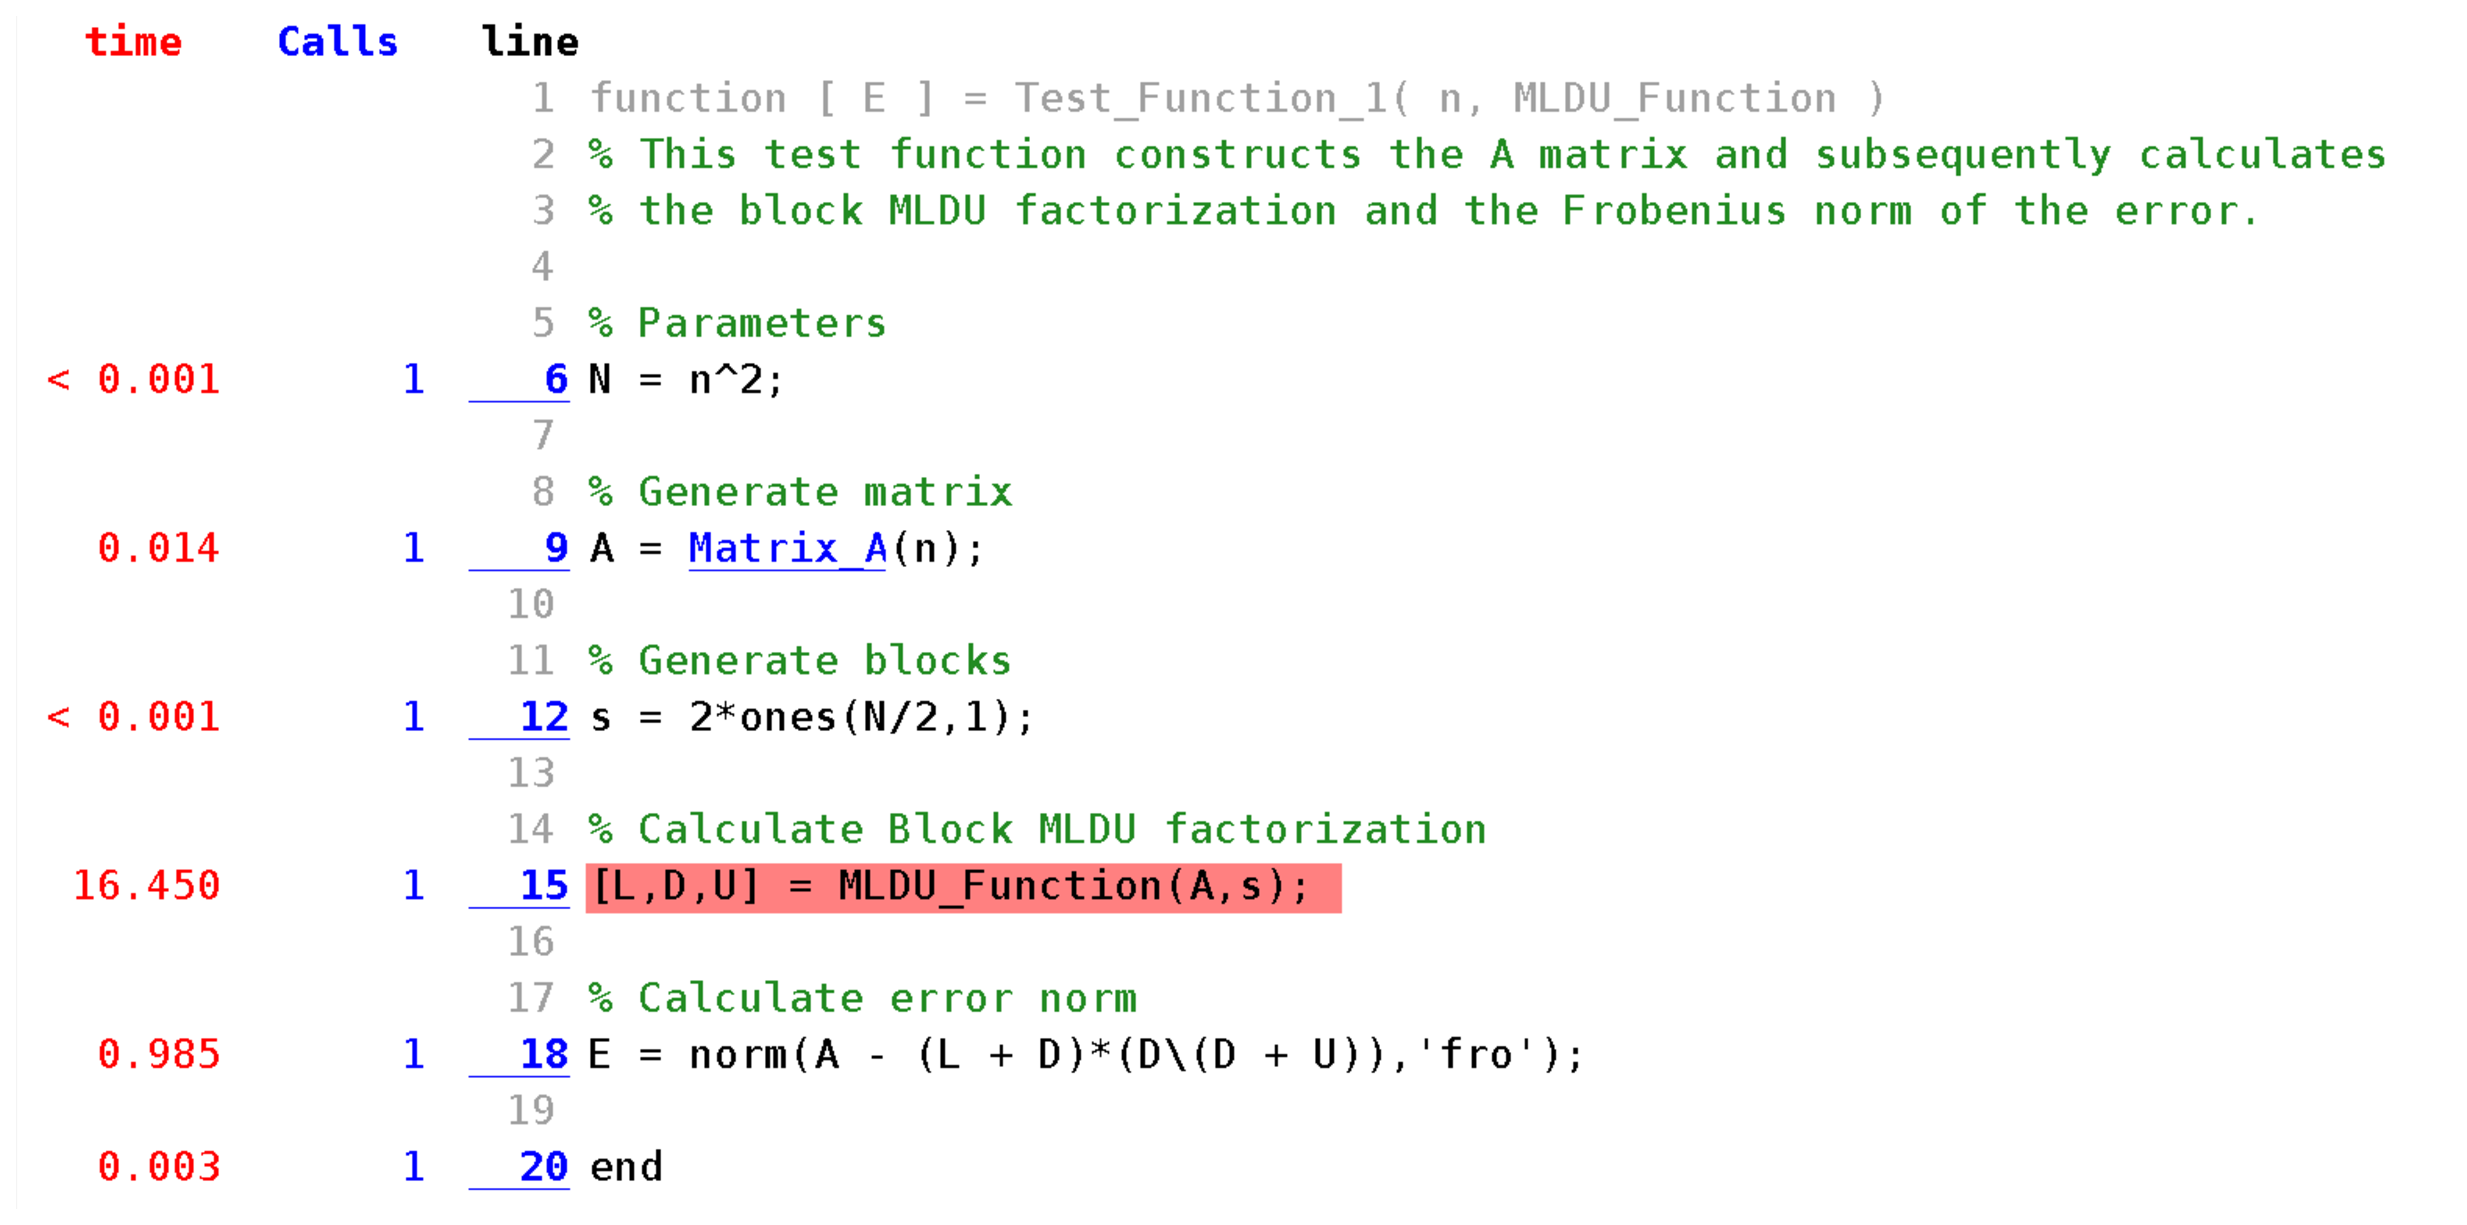
\includegraphics[width=\linewidth]{figures/Profile_MLDU_Simple_cell_1.eps}
    \centering
\end{figure}

\noindent This is exactly the same as the previous situation. The error is also acceptable:\\

\noindent \texttt{E =}\\
\\
\noindent \texttt{   1.1287e-13}\\

\noindent Apart from the targeted result that the memory consumption has decreased, a couple of other noteworthy positive changes occurred as well.\\

\noindent One of the positive aspect is that calculating the error has a vastly reduced runtime, from about $10$ seconds to just under one second. This is caused by the fact that matrices \texttt{L}, \texttt{D} and \texttt{U} are now sparse, making the calculation a lot faster.

\begin{figure}[h!]
    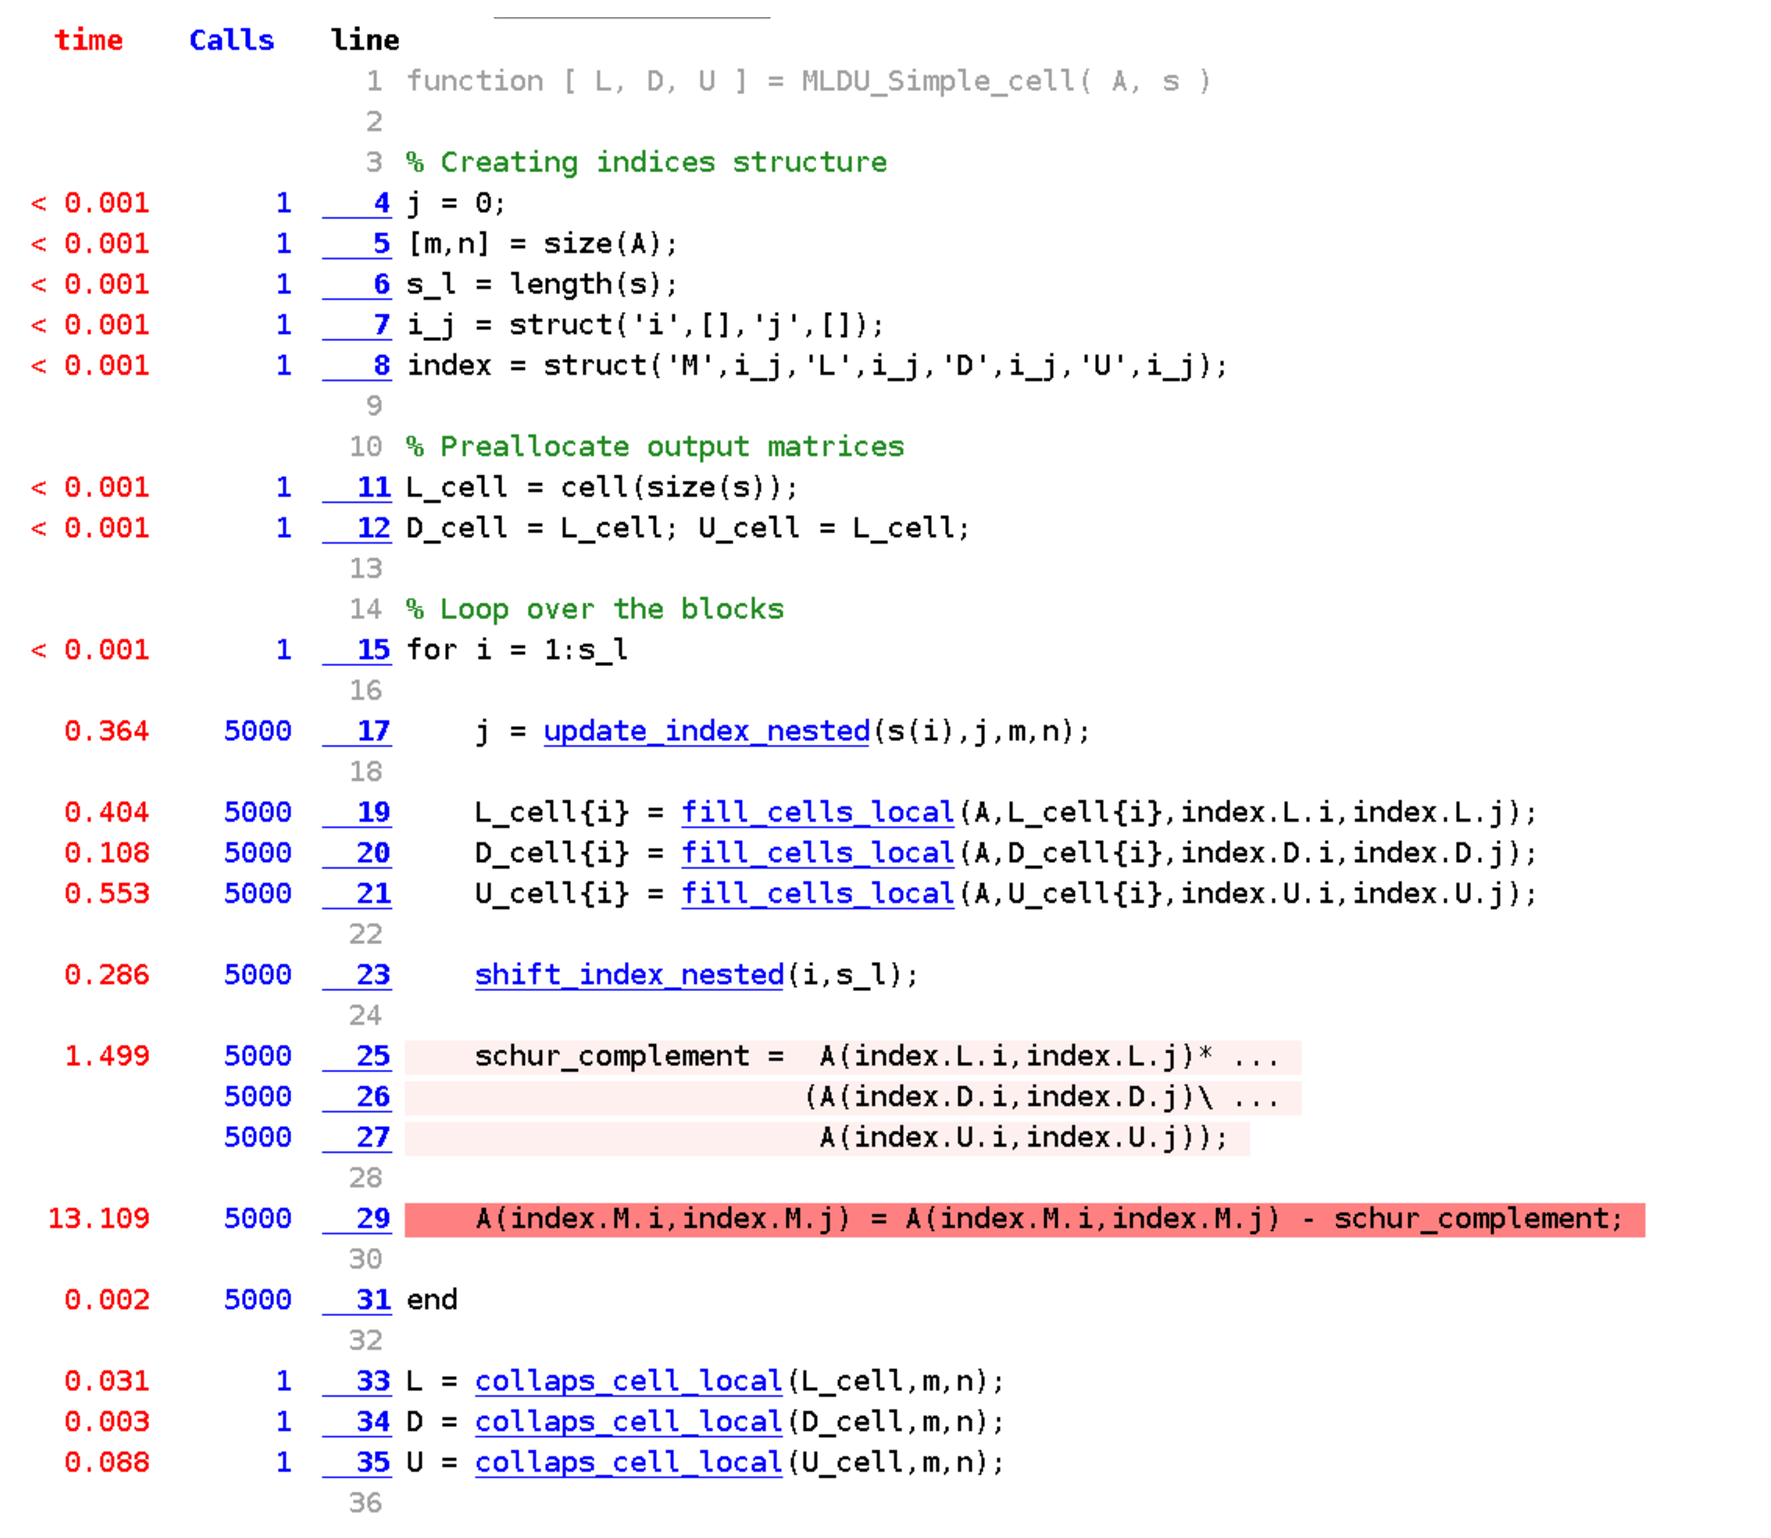
\includegraphics[width=\linewidth]{figures/Profile_MLDU_Simple_cell_2.eps}
    \centering
\end{figure}

\noindent The runtime required to save the matrices \texttt{L}, \texttt{D} and \texttt{U} has actually decreased. The initial implementation spends $2.243$ seconds at lines $19$ through $21$ while the cell array implementation takes a total of $1.187$ seconds at lines $19, 20, 21$ and $33, 34, 35$.\\

\noindent Lastly and maybe the most significant side effect of the cell array implementation is the runtime reduction of line $26$, from about $17$ seconds to about $13$ seconds, a reduction of about $25 \%$. This is probably caused by the reduced memory consumption itself, allowing the cache of the CPU to operate more effectively.